% Multijet balance: three ways to treat the MC recoil (R = 0.4)
\documentclass[aspectratio=169,10pt]{beamer}
\usepackage[T1]{fontenc}
\usepackage[utf8]{inputenc}
\usepackage{booktabs}
\usepackage{graphicx}
\usepackage{amsmath}
\setbeamertemplate{navigation symbols}{}
\setbeamertemplate{footline}{\hfill\insertframenumber\,/\,\inserttotalframenumber\hspace{1em}\vspace{0.6em}}
\newcommand{\xj}{x_{j}}

\title{Multijet balance: smearing the recoil in MC}
\subtitle{Four configurations, R = 0.4}
\author{Samuel F.\ Liechty}
\date{October 7, 2026}

\begin{document}

\begin{frame}
  \titlepage
\end{frame}

\begin{frame}{Common setup}
  \begin{itemize}
    \item $\xj = p_{T,\mathrm{lead}} / |\vec p_{T,2} + \vec p_{T,3}|$; the recoil is $|\vec p_{T,2} + \vec p_{T,3}|$.
    \item Reprocessed data and Pythia8 trees (new skim, per-event seeded JER smearing).
    \item MC: Jet12, Jet20, Jet30; Jet12 starts at truth $p_T = 0$.
    \item Leading reco jet capped at 35 GeV in Jet12 and 50 GeV in Jet20.
    \item Leading jet $\geq 20$ GeV, jets 2 and 3 $\geq 7$ GeV each, $|\eta| < 0.7$, $\Delta\phi_{12} > 3\pi/4$, $\Delta\phi_{13} > \pi/2$.
    \item Leading-$p_T$ bins 20--25, 25--30, 30--35, 35--50 GeV.
    \item MC reweighted in leading $p_T$ and $z$ vertex; two passes.
    \item Only the treatment of the MC recoil changes between the configurations.
  \end{itemize}
\end{frame}

\begin{frame}{Why the leading reco jet is capped in Jet12 and Jet20}
  \begin{columns}[T]
    \begin{column}{0.71\textwidth}
      \includegraphics[width=\linewidth,page=7]{figs/xj_samples_5bins.pdf}
    \end{column}
    \begin{column}{0.28\textwidth}
      \footnotesize
      \begin{itemize}
        \item R = 0.4 MC by sample, before the caps, with a 50--70 GeV bin.
        \item 35--50 GeV: Jet12 is 1.7\% of the MC from 2 events ($\xj \approx 1.4$, 2.3).
        \item 50--70 GeV: Jet20 is 6.9\% of the MC from 5 events ($\xj = 1.5$--1.8); data has 11 events.
        \item The spikes are a few events with large weights.
        \item Caps: leading reco jet $\leq 35$ GeV in Jet12, $\leq 50$ GeV in Jet20; the 50--70 GeV bin is dropped.
      \end{itemize}
    \end{column}
  \end{columns}
\end{frame}

\begin{frame}{After the caps (configuration 4)}
  \begin{columns}[T]
    \begin{column}{0.71\textwidth}
      \includegraphics[width=\linewidth,page=7]{figs/xj_samples_cfg4.pdf}
    \end{column}
    \begin{column}{0.28\textwidth}
      \footnotesize
      \begin{itemize}
        \item The 35--50 GeV bin is now Jet20 and Jet30 only and is smooth.
        \item Jet12 still contributes 8.7\% at 30--35 GeV from 32 events.
        \item Those events are spiky, but the total MC still follows the data.
      \end{itemize}
    \end{column}
  \end{columns}
\end{frame}

\begin{frame}{The four configurations}
  \centering
  \begin{tabular}{llll}
    \toprule
    & jets 2 and 3 & recoil smearing & recoil cut \\
    \midrule
    1 & each smeared on its own & none & none \\
    2 & each smeared on its own & none & $\geq 14$ GeV \\
    3 & added unsmeared & sum smeared once, every event & $\geq 14$ GeV \\
    \midrule
    4 & one truth jet: added unsmeared & one truth jet: sum smeared once & $\geq 14$ GeV \\
            & otherwise: each smeared on its own & otherwise: none & \\
    \bottomrule
  \end{tabular}
  \vspace{1em}
  \begin{itemize}
    \item In configuration 3 the smearing width is taken at the unsmeared recoil $p_T$, so truth is used only for the sample stitching.
    \item Configuration 4 smears the recoil only when jets 2 and 3 belong to a single truth jet (next slide), with the width at that truth jet's $p_T$.
    \item Its other events smear jets 2 and 3 individually, as in configuration 2.
    \item The 7 GeV jet cuts use the values before any recoil smearing.
  \end{itemize}
\end{frame}

\begin{frame}{Configuration 4: are jets 2 and 3 one truth jet?}
  \begin{itemize}
    \item Truth jets $\geq 7$ GeV; reco jets ranked by calibrated $p_T$; matching radius $0.75R$.
    \item The leading jet matches a truth jet $T_L$ (stored match, else the nearest truth jet).
    \item Jet 2 matches its nearest truth jet $T_R \neq T_L$.
    \item Jet 3 matches $T_R$ or no truth jet, never $T_L$.
    \item Every other truth jet is more than $1.5R$ from jets 2 and 3.
    \item The summed recoil $\vec p_{T,2} + \vec p_{T,3}$ lies within $0.75R$ of $T_R$.
  \end{itemize}
  \vspace{0.5em}
  \begin{itemize}
    \item If all hold, the sum is smeared once with the width at $p_T(T_R)$, and jets 2 and 3 are scaled to the smeared recoil.
    \item Otherwise jets 2 and 3 are smeared individually.
    \item At R = 0.4 about 32\% of the weighted selected MC gets the recoil smearing (22\% with truth jets $\geq 5$ GeV).
  \end{itemize}
\end{frame}

\begin{frame}{Result: data/MC of $\langle \xj \rangle$, R = 0.4}
  \centering
  \small
  \begin{tabular}{lcccc}
    \toprule
    & 20--25 & 25--30 & 30--35 & 35--50 \\
    \midrule
    1: individual, no recoil cut & 1.019 $\pm$ 0.003 & 1.025 $\pm$ 0.005 & 1.020 $\pm$ 0.008 & 1.031 $\pm$ 0.011 \\
    2: individual, recoil cut & 1.026 $\pm$ 0.003 & 1.031 $\pm$ 0.005 & 1.020 $\pm$ 0.008 & 1.030 $\pm$ 0.011 \\
    3: recoil smeared, all events & 0.998 $\pm$ 0.004 & 0.990 $\pm$ 0.005 & 0.979 $\pm$ 0.007 & 0.980 $\pm$ 0.011 \\
    4: smeared if one truth jet & 0.999 $\pm$ 0.003 & 0.995 $\pm$ 0.005 & 0.981 $\pm$ 0.008 & 0.988 $\pm$ 0.011 \\
    4, truth jets $\geq 5$ GeV & 1.006 $\pm$ 0.003 & 0.999 $\pm$ 0.005 & 0.990 $\pm$ 0.008 & 0.993 $\pm$ 0.011 \\
    hybrid: 3 with truth width & 1.000 $\pm$ 0.004 & 0.991 $\pm$ 0.005 & 0.979 $\pm$ 0.007 & 0.980 $\pm$ 0.011 \\
    \midrule
    data events & 16090 & 5346 & 1640 & 590 \\
    \bottomrule
  \end{tabular}
  \vspace{1em}
  \begin{itemize}
    \item The recoil cut removes about 1.5\% of data events and moves the ratio by at most 0.007.
    \item Smearing the summed recoil once raises the MC $\langle\xj\rangle$ by 2.5--5\%.
    \item Hybrid (configuration 3 with the truth width in two-truth-jet events) matches configuration 3, so the width choice does not matter.
  \end{itemize}
\end{frame}

\begin{frame}{Configuration 1: individual smearing, no recoil cut}
  \begin{columns}[T]
    \begin{column}{0.62\textwidth}
      \includegraphics[width=\linewidth,page=7]{figs/dists_cfg1.pdf}
    \end{column}
    \begin{column}{0.36\textwidth}
      \includegraphics[width=\linewidth,page=7]{figs/means_cfg1.pdf}
    \end{column}
  \end{columns}
  \vspace{0.3em}
  \begin{itemize}
    \item Data lies 2--3\% above MC in every bin.
    \item The MC $\xj$ distribution peaks slightly lower than data.
  \end{itemize}
\end{frame}

\begin{frame}{Configuration 2: individual smearing, recoil $\geq 14$ GeV}
  \begin{columns}[T]
    \begin{column}{0.62\textwidth}
      \includegraphics[width=\linewidth,page=7]{figs/dists_cfg2.pdf}
    \end{column}
    \begin{column}{0.36\textwidth}
      \includegraphics[width=\linewidth,page=7]{figs/means_cfg2.pdf}
    \end{column}
  \end{columns}
  \vspace{0.3em}
  \begin{itemize}
    \item Nearly identical to configuration 1.
    \item Two jets of at least 7 GeV almost always give a recoil above 14 GeV.
  \end{itemize}
\end{frame}

\begin{frame}{Configuration 3: add unsmeared, smear the recoil, recoil $\geq 14$ GeV}
  \begin{columns}[T]
    \begin{column}{0.62\textwidth}
      \includegraphics[width=\linewidth,page=7]{figs/dists_cfg3.pdf}
    \end{column}
    \begin{column}{0.36\textwidth}
      \includegraphics[width=\linewidth,page=7]{figs/means_cfg3.pdf}
    \end{column}
  \end{columns}
  \vspace{0.3em}
  \begin{itemize}
    \item The distributions agree over the whole $\xj$ range in the first three bins.
    \item The ratio is about 1.00 at 20--25 GeV and 0.98--0.99 above.
  \end{itemize}
\end{frame}

\begin{frame}{Configuration 4: recoil smearing when jets 2 and 3 are one truth jet}
  \begin{columns}[T]
    \begin{column}{0.62\textwidth}
      \includegraphics[width=\linewidth,page=7]{figs/dists_cfg4.pdf}
    \end{column}
    \begin{column}{0.36\textwidth}
      \includegraphics[width=\linewidth,page=7]{figs/means_cfg4.pdf}
    \end{column}
  \end{columns}
  \vspace{0.3em}
  \begin{itemize}
    \item Jets 2 and 3 from one truth jet: added unsmeared, the sum smeared at that truth jet's $p_T$.
    \item All other events: jets 2 and 3 smeared individually.
    \item The ratio is 1.00 at 20--30 GeV and 0.98--0.99 above.
  \end{itemize}
\end{frame}

\begin{frame}{Summary}
  \begin{itemize}
    \item How the recoil is smeared, not the recoil cut, sets the data/MC agreement.
    \item Smearing jets 2 and 3 individually leaves a 2--3\% data excess.
    \item Adding jets 2 and 3 unsmeared and smearing the sum once removes it.
    \item Adopted: configuration 4, with truth jets $\geq 7$ GeV.
    \item Its data/MC ratio is 0.999, 0.995, 0.981 and 0.988 in the four bins.
    \item Configuration 3 agrees within 0.8\%, and the hybrid shows the width choice plays no role.
    \item The 5 GeV truth-jet threshold moves the ratio by up to 0.009, a candidate systematic.
  \end{itemize}
\end{frame}

\end{document}
